\documentclass[11pt, a4paper]{article}
\usepackage[utf8]{inputenc}
\usepackage{t1enc}
\usepackage[magyar]{babel}
\usepackage{lmodern}
\usepackage{url}
\usepackage{graphics}
\usepackage{listings}
\usepackage[a4paper, total={5.3in, 8in}]{geometry}

\sloppy

\begin{document}
\title{Szoftver architektúrák \\ Szótanulást segítő alkalmazás \\ \large{Rendszerterv}}
    \author{Graics Bence \and Verbőczy Kristóf}

    \maketitle
    
    \tableofcontents
    \newpage
    
    \section{Bevezetés}
    \label{sec:bevezetes}
    Jelen dokumentum a Szoftver architektúrák nevű tárgyra kidolgozott házi feladat rendszertervet mutatja be. A házi feladat során a cél egy szótanulást segítő alkalmazás megtervezése és implementálása volt. A követelmények és a specifikáció a ... érhető el.
    
    A dokumentum a következők szerint épül fel:
    
    \section{Architektúra}
    \label{sec:architektúra}
    Jelen fejezet bemutatja az elkészített szótanuló alkalmazás architektúráját, azaz hogy \textit{1)} a rendszer milyen komponensekből épül fel, \textit{2)} az egyes komponenseknek milyen lényeges elemei vannak, \textit{3)} a komponensek hogyan kapcsolódnak egymáshoz.
    
    Az általunk tervezett rendszer egy adatközpontú alkalmazás, amely kliens-szerver architektúrát követ. A szerver tárolja a szükséges adatokat, például a felhasználók adatait és az egyes leckékhez tartozó adatokat (szavakat és képeket). A kliens feladata, hogy a felhasználó kérésére fogyasztható formában tárja a felhasználó elé ezen adatokat, és kezelje az esetleges interakciókat. Az adatok (az objektum-orientáltság szabályai szerint) objektumokban (DTO) kerülnek továbbításra és feldolgozásra. A szerver és a kliens kommunikációját jól meghatározott interfészek teszik lehetővé.
    
    \subsection{Objektumok}
    
    \subsection{Interfészek}
    
    \subsection{A szerver}
    A szerver architektúrája négy fő részre bontható. Ezek az alábbiak:
    \begin{itemize}
    	\item szolgáltatás hozzáférési réteg (Rest API),
    	\item üzleti logika réteg,
    	\item adatelérési réteg,
    	\item adatbázis réteg.
    \end{itemize}
    A közöttük lévő kapcsolatot mutatja be \aref{fig:server_arch}. ábra.
    
    \begin{figure}[htbp]
    	\center
    	\resizebox{140mm}{!}{
    		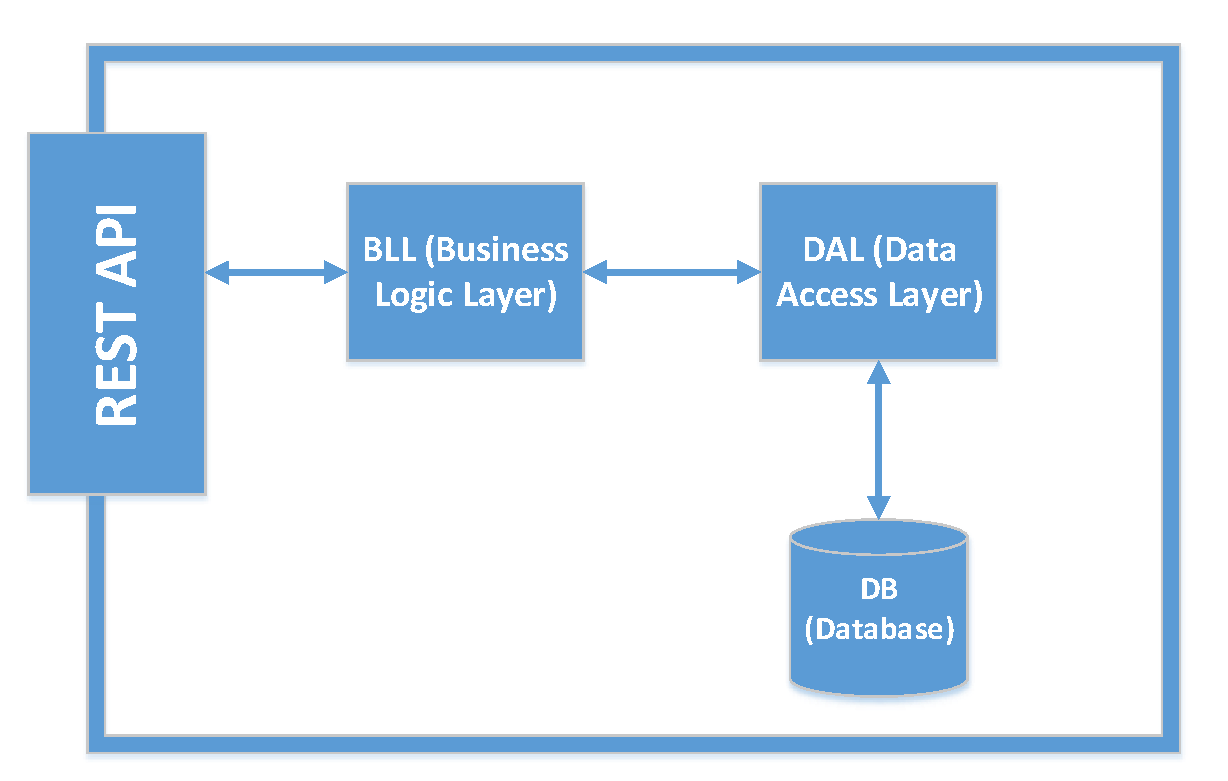
\includegraphics{figures/server_architecture.pdf}
    	}
    	\caption{A szerver architekturális felépítése}
    	\label{fig:server_arch}
    \end{figure}
    
    \subsubsection{Szolgáltatás hozzáférési réteg}
    Az a réteg egy REST API-nak felel meg, amelyen keresztül http kérésekkel és erre adott http válaszokkal lehet igénybe venni a szerver szolgáltatását. Az előző \textit{Interfészek} fejezet ezt írta le részletesen, ezért itt nem kerül megismétlésre.
    
    \textbf{Megjelenés a kódban:} \textit{language.learning.server} package-ben található interfészek: 
    \begin{itemize}
    	\item ILearning
    	\item IExerciseManager
    	\item IUserManager
    \end{itemize}
    
    A fejlesztés során lehetőség volt a program kliens nélküli tesztelésére, hiszen elég http kéréseket küldeni neki. Erre a \textit{Postman} nevezetű programot használtuk.
    
    \subsubsection{Üzleti logika réteg}
    Ez a réteg tulajdonképpen a szolgáltatás interfészek konkrét megvalósításaiból áll. Feladata adatelérési réteg megfelelő metódusainak meghívása, és az eredmény az interfészben definiált formára hozása. Erre jó példa, hogy véletlenszerűen kell visszaadnia a szervernek N darab feladatot, ahol N-t a kliens kérése határozza meg. Ez a feladat tipikusan üzleti logika hatáskörébe tartozik.
    
    \textbf{Megjelenés a kódban:} \textit{language.learning.server} package-ben található osztályok: 
    \begin{itemize}
    	\item Learning
    	\item ExerciseManager
    	\item UserManager
    \end{itemize}
    
    \subsubsection{Adatelérési réteg}
    Feladata az adatbázishoz való hozzáférés, melynek során biztosítja a szükséges \textit{lekérdezéseket, beszúrásokat, módosításokat, törléseket}. Ezen a szinten történik a védekezés az SQL injection ellen, a \textit{java.sql.PreparedStatement} interfész segítségével.
    
    \textbf{Megjelenés a kódban:} \textit{language.learning.database} package-ben IDatabase interfész, és ennek a megvalósítása a Database osztály.
    
    Az adatbázis elérésére az Oracle jdbc drivere került felhasználásra, ezt a kódban a Database osztályban meg is kell adni.
    
    \subsubsection{Adatbázis réteg}
    Feladata az adatok perzisztens tárolása. A használt adatbázis az Oracle Database11g Express Edition. Azért erre esett a választás, mert ingyenes, és mivel korábbi tapasztalataink az Oracle adatbázisokhoz voltak köthetők, ezért mindenféleképpen Oracle terméket szerettünk volna használni. Bár vannak újabb verziók is, de azokat nem sikerült telepíteni, ezért maradt a 11g verzió.
    
    Megjelenés a kódban: nem írtunk hozzá komponenst, viszont a függőségek között megjelenik az ojdbc7.jar, ami szintén ingyenesen letölthető az Oracle honlapjáról. Érdekesség, hogy a projektünk Maven projekt, így a pom.xml-be megadott függőségek automatikusan letöltődnek, viszont az Oracle nem teszi ki publikus repository-ba az ojdbc driver-t, ezért manuálisan kell letölteni és beállítani a függőségeket.
    
    \subsection{Adatbázis terv}
    Ezen fejezetben bemutatásra kerülnek az adatbázisban elmentett entitások. Az adatbázis (nem teljesen szabványos) egyed-kapcsolat diagramja látható \aref{fig:er_diag}. ábrán.
    
    \begin{figure}[htbp]
    	\center
    	\resizebox{140mm}{!}{
    		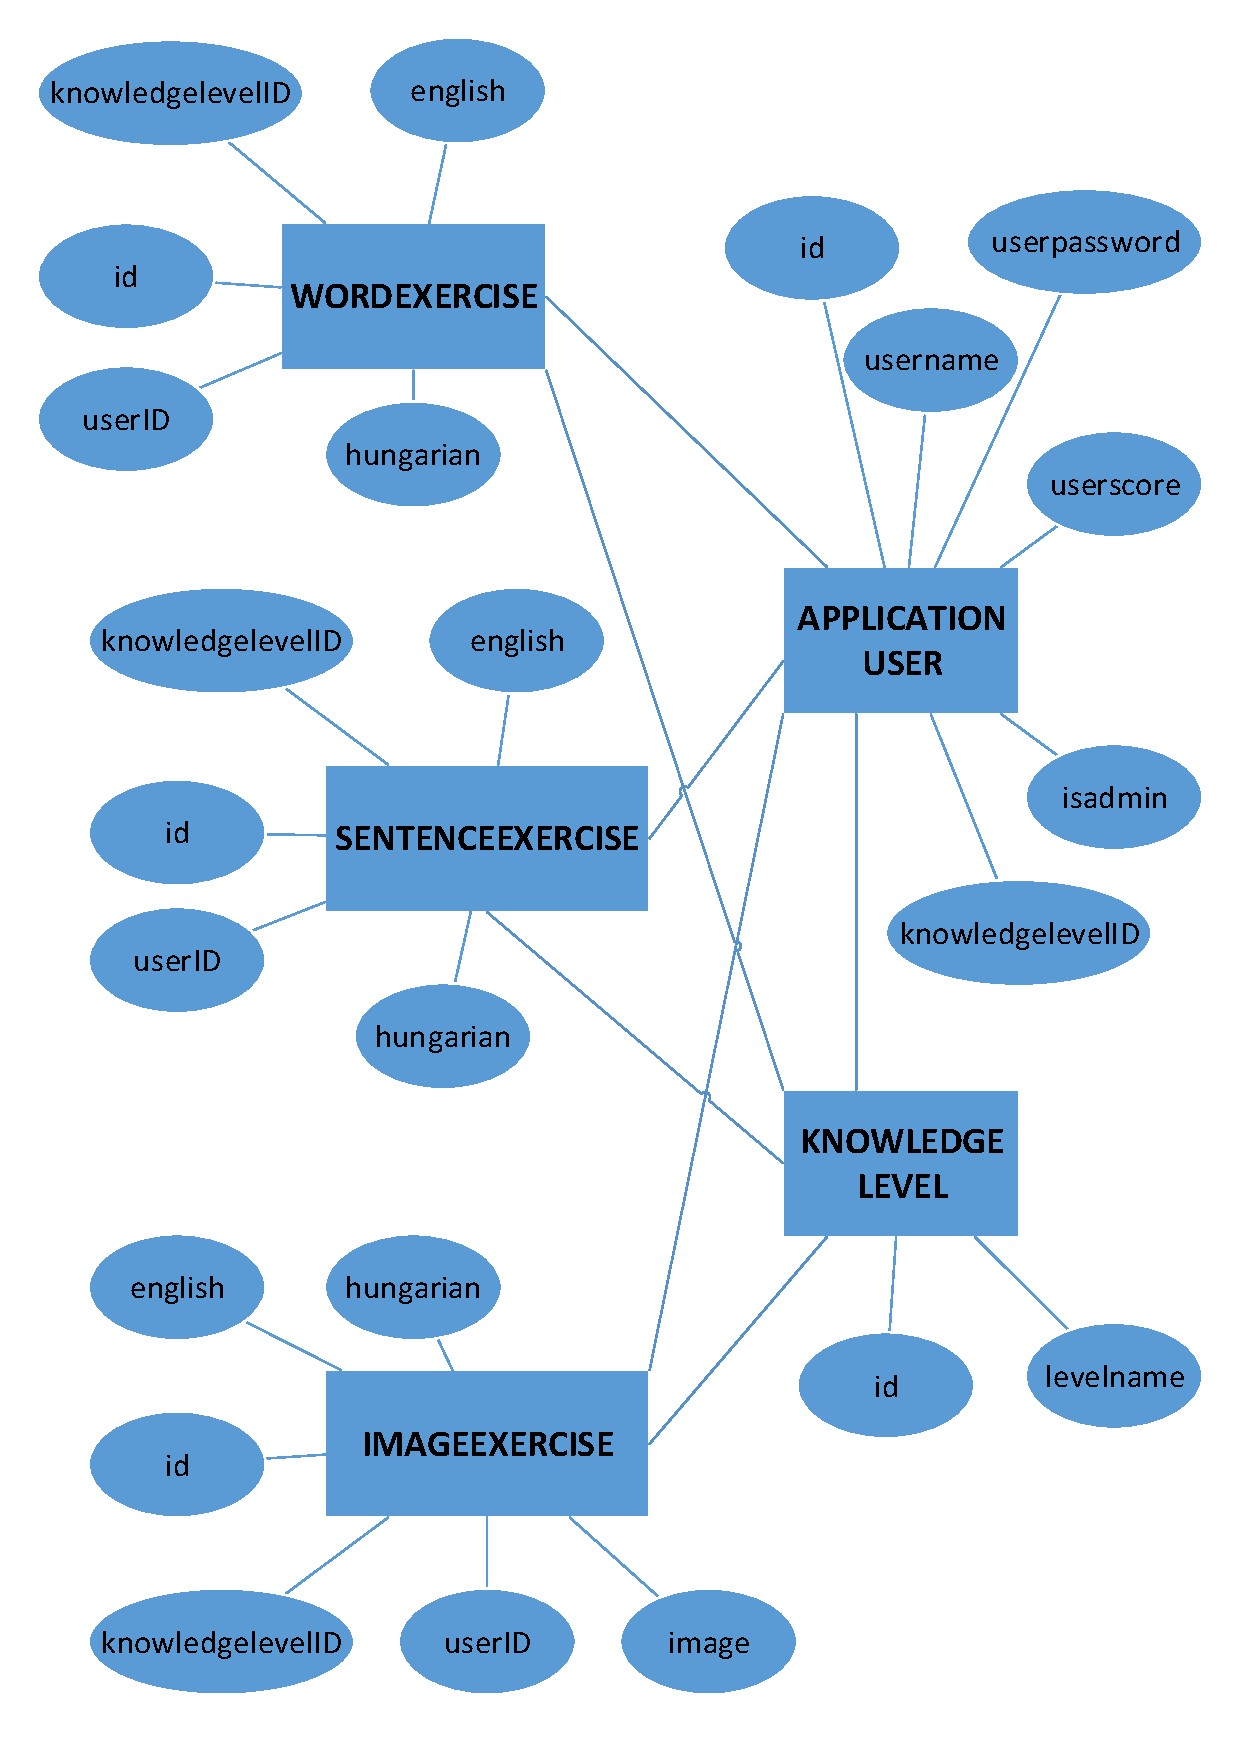
\includegraphics{figures/er.pdf}
    	}
    	\caption{A szerver architekturális felépítése}
    	\label{fig:er_diag}
    \end{figure}
    
    \subsubsection{WORDEXERCISE}
    A szó feladatokhoz szükséges adatok tárolására alkalmas. Egy szópárt tárol, ami egyébként könnyedén kibővíthető új nyelvekkel. Továbbá tárolja, hogy milyen nehézségű a feladat, és azt is, hogy melyik felhasználó hozta létre.
    
    Az id értékének generálására a \textit{WORDEXERCISE\_SEQ} szekvencia szolgál.
    
    \begin{table}[!h]
    	\centering
    	\begin{tabular} {|c|c|c|}
    		\hline
    		Név & Adatbázis típus & Java típus \\
    		\hline
    		id & number \textbf{(PK)} & nem jelenik meg ez a mező \\
    		english & nvarchar2(30) & String \\
    		hungarian & nvarchar2(30) & String \\
    		userid & number \textbf{(FK)} & int \\
    		knowledgelevelID & number \textbf{(FK)} & int \\
    		\hline
    	\end{tabular}
    \end{table}
    
    \subsubsection{SENTENCEEXERCISE}
    Nagyon hasonlít a \textit{WORDEXERCISE}-ra, de ez alkalmas hosszabb karakterlánc párok eltárolására is, tehát nem csak szavakat, hanem hosszabb mondatokat is tudunk tárolni benne. Elképzelhetőnek tartom, hogy össze lehetne vonni a \textit{WORDEXERCISE} és \textit{SENTENCEEXERCISE} táblákat, de akkor szükség lenne a típus bevezetésére, továbbá így érthetőbb miképp válnak külön a feladattípusok.
    
    Az id értékének generálására a \textit{SENTENCEEXERCISE\_SEQ} szekvencia szolgál.
    
    \begin{table}[!h]
    	\centering
    	\begin{tabular} {|c|c|c|}
    		\hline
    		Név & Adatbázis típus & Java típus \\
    		\hline
    		id & number \textbf{(PK)} & nem jelenik meg ez a mező \\
    		english & nvarchar2(200) & String \\
    		hungarian & nvarchar2(200) & String \\
    		userid & number \textbf{(FK)} & int \\
    		knowledgelevelID & number \textbf{(FK)} & int \\
    		\hline
    	\end{tabular}
    \end{table}
    
    \subsubsection{IMAGEEXERCISE}
    Annyiban különbözik a \textit{WORDEXERCISE}-tól, hogy képes képek tárolására. Az id értékének generálására az \textit{IMAGEEXERCISE\_SEQ} szekvencia szolgál.
    
    \begin{table}[!h]
    	\centering
    	\begin{tabular} {|c|c|c|}
    		\hline
    		Név & Adatbázis típus & Java típus \\
    		\hline
    		id & number \textbf{(PK)} & nem jelenik meg ez a mező \\
    		english & nvarchar2(30) & String \\
    		hungarian & nvarchar2(30) & String \\
    		userid & number \textbf{(FK)} & int \\
    		knowledgelevelID & number \textbf{(FK)} & int \\
    		image & BLOB & byte[] \\
    		\hline
    	\end{tabular}
    \end{table}
    
    \subsubsection{APPLICATIONUSER}
    A felhasználó adatait tárolja. Az egyértelmű felhasználónév, jelszón kívül még a pontszámát, a tudásszintjét és azt, hogy rendelkezik-e adminisztrátori jogosultsággal.
    
    Az id értékének generálására a \textit{USER\_SEQ} szekvencia szolgál.
    
    \begin{table}[!h]
    	\centering
    	\begin{tabular} {|c|c|c|}
    		\hline
    		Név & Adatbázis típus & Java típus \\
    		\hline
    		id & number \textbf{(PK)} & nem jelenik meg ez a mező \\
    		username & nvarchar2(15) & String \\
    		userpassword & nvarchar2(128) & String \\
    		userscore & number & int \\
    		knowledgelevelID & number \textbf{(FK)} & int \\
    		isadmin & number & boolean \\
    		\hline
    	\end{tabular}
    \end{table}
    
    \subsubsection{KNOWLEDGELEVEL}
    A különböző tudásszinteket tárolja. Mivel ezt a felhasználók nem tudják befolyásolni és kevés típus van, ezért nem szükséges szekvencia az id értékének generálására.
    
    \begin{table}[!h]
    	\centering
    	\begin{tabular} {|c|c|c|}
    		\hline
    		Név & Adatbázis típus & Java típus \\
    		\hline
    		id & number \textbf{(PK)} & nem jelenik meg ez a mező \\
    		levelname & nvarchar2(10) & enumeráció \\
    		\hline
    	\end{tabular}
    \end{table}
    
    \subsection{A kliens}
    \label{sec:kliens}
    A kliens a következő feladatokat látja el, felhasználva a szerver által nyújtott szolgáltatásokat.
    \begin{enumerate}
    	\item Megjelenít különböző adatokat. Ezen adatok tartozhatnak egy adott felhasználóhoz, pl.~név, pontszám, tudásszint, vagy tartozhat leckékhez, pl. angol szó, magyar szó, objektumot leíró kép.
    	\item Felhasználói kéréseket hajt végre az alkalmazáslogikának megfelelően. Ezek közé tartozik egy lecke megtanítása (tanítási folyamat végrehajtása), leckék kilistázása, leckék felvétele és törlése, felhasználók létrehozása és törlése (adminisztrátor felhasználó esetén).
    	\item A felhasználói kérések teljesítéséhez felveszi a kapcsolatot a szerverrel, hogy lekérje a szükséges adatokat, illetve perzisztálja adatok módosításának az eredményét.
    \end{enumerate}

	A kliens egy réteges felépítést követ, minden réteghez egy fent meghatározott feladat társul. A kliens felépítését \aref{fig:client-arch}.~ábra mutatja be.
	       \begin{figure}[htbp]
	       	\center
	       	\resizebox{60mm}{!}{
	       		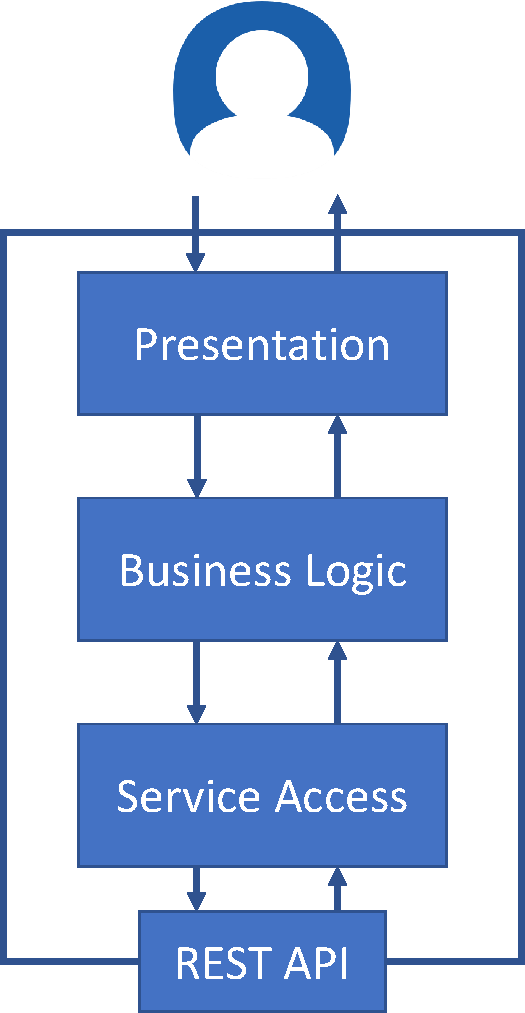
\includegraphics{figures/client-arch.pdf}
	       	}
	       	\caption{A kliens architektúrája.}
	       	\label{fig:client-arch}
	       \end{figure}
	
	Amint látható, a kliens egy tisztán rétegelt architektúrát valósít meg. A megjelenítési réteg csak az üzleti logikai réteg  nyújtotta szolgáltatásokat használja fel, az üzleti logikai réteg pedig csak a szolgáltatás hozzáférési rétegre támaszkodik. Az alkalmazásban egy réteget egy osztály valósít meg. A következő szekciók részletesebben bemutatják az egyes rétegek megvalósítását.
     
     \subsubsection{Megjelenítési réteg: View osztály}
     A View osztály felelős a grafikus felhasználói felület megvalósításáért. A grafikus felület a JavaFX FXML technológia felhasználásával került definiálásra. Ennek segítségével a felületen található vezérlőket deklaratív jelleggel lehet definiálni az XML szintaktikának megfelelően: vezérlő hierarchiákat lehet létrehozni, illetve az egyes vezérlők tulajdonságait lehet definiálni (méret, szín, elrendezési algoritmus). A következő kódrészlet a bejelentkezéshez szükséges vezérlők definiálását mutatja be.
     
\begin{lstlisting}[
basicstyle=\small, %or \small or \footnotesize etc.
]
<HBox fx:id="connectionLayout" alignment="CENTER_LEFT"
	spacing="10">
<!-- Username field -->
<TextField fx:id="userNameField" maxWidth="200" maxHeight="27"
minWidth="100" minHeight="28" prefWidth="200" prefHeight="27" 
	promptText="User name" />	
<!-- Password field -->
<PasswordField fx:id="passwordField" prefWidth="200" 
	prefHeight="27" promptText="Password" />	
<Pane HBox.hgrow="ALWAYS" />
<!-- Connect button -->			
<Button fx:id="connectButton" text="Connect" prefWidth="100" 
	onAction="#connectEventHandler" />
</HBox>
\end{lstlisting}
     
     A grafikus felület egy \emph{egyablakos} megközelítést követ; az egyes funkciók különböző \emph{füleken} keresztül érhetők el. A következőkben bemutatjuk a legfontosabb képernyőket, amelyek az alkalmazás jelentősebb funkcionalitásaihoz tartoznak.
     
     A program indulása utána a következő képernyő fogad (lásd \ref{fig:connect}.~ábra).     
     \begin{figure}[htbp]
	     \center
	     \resizebox{110mm}{!}{
		     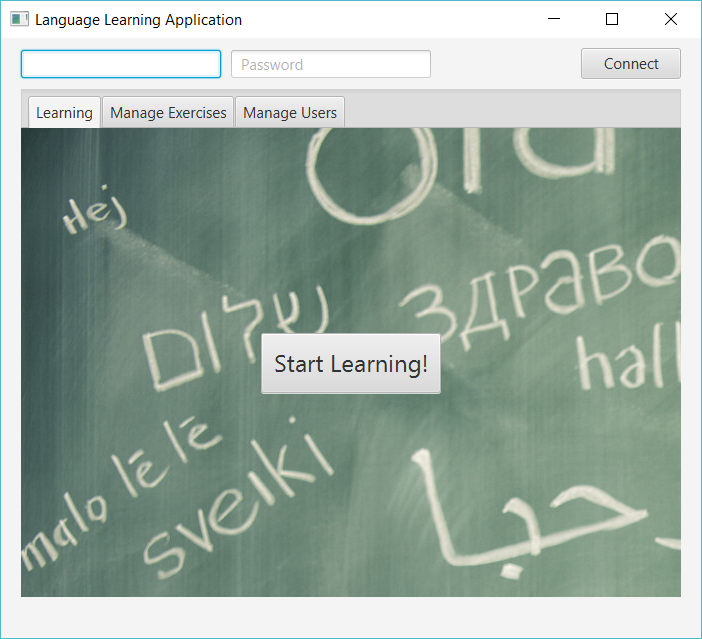
\includegraphics{figures/connect.png}
	     }
	     \caption{A bejelentkező képernyő.}
	     \label{fig:connect}
     \end{figure} 
     Ekkor a felhasználónak lehetősége van bejelentkezni. Rossz felhasználónév vagy jelszó esetén az alkalmazás egy felugró ablakkal figyelmeztet (\ref{fig:login-error}.~ábra).
     \begin{figure}[htbp]
     	\center
     	\resizebox{80mm}{!}{
     		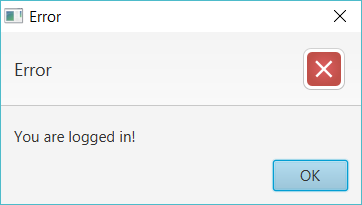
\includegraphics{figures/login-error.png}
     	}
     	\caption{Rossz felhasználónév vagy jelszó esetén hibaüzenet.}
     	\label{fig:login-error}
     \end{figure}
     Bejelentkezés után a felhasználó megvizsgálhatja jelenlegi pontjait, tudás szintjét, illetve ki is jelentkezhet (\ref{fig:after-connect}.~ábra).     
     \begin{figure}[htbp]
     	\center
     	\resizebox{110mm}{!}{
     		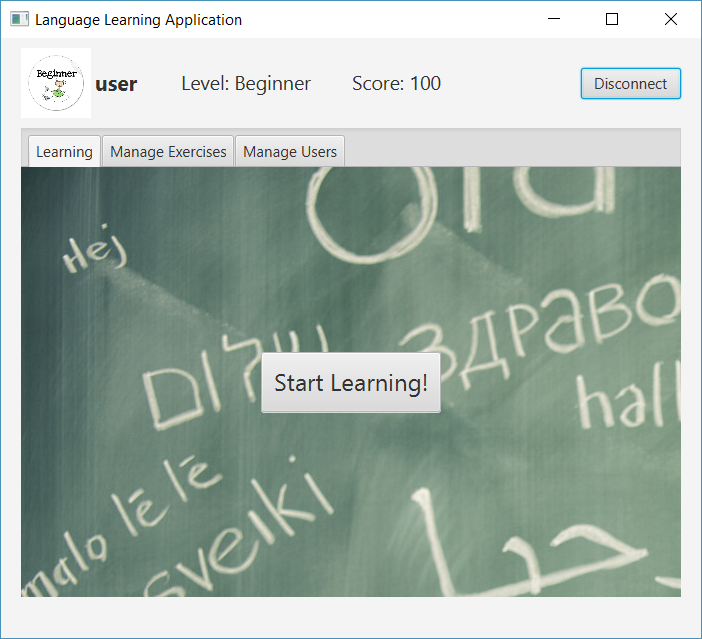
\includegraphics{figures/after-connect.png}
     	}
     	\caption{A kezdőablak bejelentkezés után.}
     	\label{fig:after-connect}
     \end{figure}
     A tanulást, azaz egy lecke megkezdését a \emph{Start Learning!} gombra kattintva kezdheti el, ahol a három különböző feladattípushoz a következő képernyők tartoznak (\ref{}, \ref{} és \ref{} ábra).
     %       \begin{figure}[htbp]
     %       	\center
     %       	\resizebox{140mm}{!}{
     %       		\includegraphics{messageformat.pdf}
     %       	}
     %       	\caption{Chat üzenet formátum}
     %       	\label{fig:messageformat}
     %       \end{figure}
     %       \begin{figure}[htbp]
     %       	\center
     %       	\resizebox{140mm}{!}{
     %       		\includegraphics{messageformat.pdf}
     %       	}
     %       	\caption{Chat üzenet formátum}
     %       	\label{fig:messageformat}
     %       \end{figure}
     %       \begin{figure}[htbp]
     %       	\center
     %       	\resizebox{140mm}{!}{
     %       		\includegraphics{messageformat.pdf}
     %       	}
     %       	\caption{Chat üzenet formátum}
     %       	\label{fig:messageformat}
     %       \end{figure}
     Leckék kezelését (hozzáadás, törlés, listázás) a felhasználó a \emph{Manage Exercises} fülön végezheti (\ref{fig:manage-exercises}.~ábra).
     \begin{figure}[htbp]
     	\center
     	\resizebox{110mm}{!}{
     		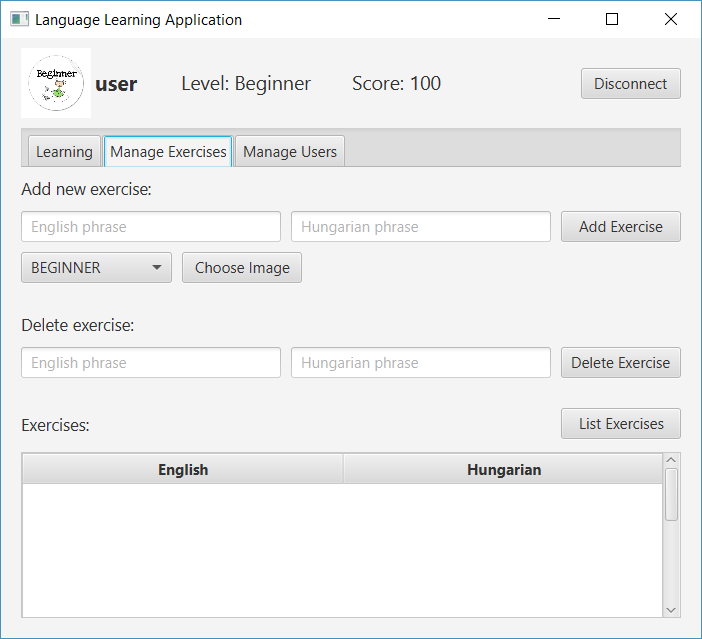
\includegraphics{figures/manage-exercises.png}
     	}
     	\caption{A leckék kezelését segítő ablak.}
     	\label{fig:manage-exercises}
     \end{figure}
     Végül a grafikus felületen található egy adminisztrációs felület is (\emph{Manage Users}), amelyet adminisztrátor felhasználók vehetnek igénybe (\ref{fig:manage-users}.~ábra). Itt lehet felhasználókat törölni, illetve új felhasználókat hozzáadni az alkalmazáshoz.
     \begin{figure}[htbp]
     	\center
     	\resizebox{110mm}{!}{
     		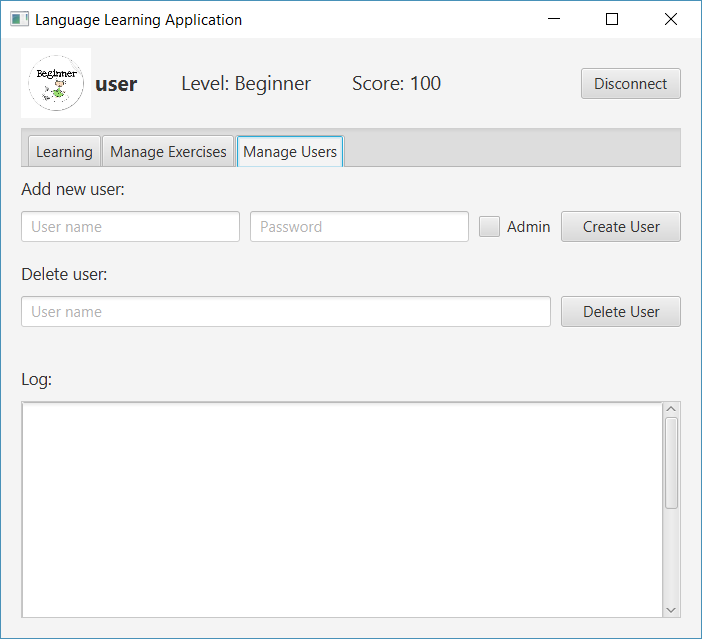
\includegraphics{figures/manage-users.png}
     	}
     	\caption{A leckék kezelését segítő ablak.}
     	\label{fig:manage-users}
     \end{figure}
   
     \subsubsection{Controller}
     A Controller felelős a felhasználói interakciók kezeléséért és az alkalmazáslogika megvalósításáért. A felhasználói interakciók lekezelése handler metódusokkal történik.
     
     Az alkalamzáslogika legbonyolultabb része a leckék levezénylésének a folyamata.
     \subsubsection{Service access}
     
    \section{Telepítési útmutató}
    
%       \begin{figure}[htbp]
%       	\center
%       	\resizebox{140mm}{!}{
%       		\includegraphics{messageformat.pdf}
%       	}
%       	\caption{Chat üzenet formátum}
%       	\label{fig:messageformat}
%       \end{figure}
    

\end{document}